\documentclass[12pt,pdf,hyperref={unicode}]{beamer}


%\documentclass[10pt]{beamer}

\usetheme[progressbar=frametitle]{metropolis}

\usepackage{booktabs}
\usepackage[scale=2]{ccicons}

\usepackage{pgfplots}
\usepgfplotslibrary{dateplot}

\usepackage{xspace}
\newcommand{\themename}{\textbf{\textsc{metropolis}}\xspace}


%\usepackage{lmodern}

% подключаем кириллицу 
\usepackage[T2A]{fontenc}
\usepackage[utf8]{inputenc}
\usepackage{listings}
%\usepackage{graphicx}
\usepackage{hyperref}

% отключить клавиши навигации
\setbeamertemplate{navigation symbols}{}

% тема оформления
\usetheme{Pittsburgh}

% цветовая схема
\usecolortheme{default}

\definecolor{light-gray}{gray}{0.90}
\definecolor{stringyellow}{RGB}{255,127,0}

\title{Семинар №6}   
\subtitle{ФАКИ \the\year}
\author{Бирюков В. А.} 
\date{\today}
% \logo{
\includegraphics[height=5mm]{images/logo.png}\vspace{-7pt}}

\begin{document}

\lstset{language=C}

% титульный слайд
\begin{frame}
\titlepage
\end{frame} 

\defverbatim[colored]\makeset{
\begin{lstlisting}[language=C++,basicstyle=\ttfamily,keywordstyle=\color{blue}]
void make_set(int X) {
  parent[X] = X;
}
\end{lstlisting}
}

\lstset{
  language=C,                % choose the language of the code
  basicstyle=\ttfamily,
  columns=fixed,
  fontadjust=true,
  basewidth=0.5em,
  keywordstyle=\color{blue}\bfseries,
  commentstyle=\color{gray},
  stringstyle=\ttfamily\color{yellow!40!red},
  showstringspaces=false,
  %numbers=false,                   % where to put the line-numbers
  numbersep=5pt,
  numberstyle=\tiny\color{gray},
  numberfirstline=true,
  stepnumber=1,                   % the step between two line-numbers.        
  numbersep=5pt,                  % how far the line-numbers are from the code
  backgroundcolor=\color{white!90!gray},  % choose the background color. You must add \usepackage{color}
  showstringspaces=false,         % underline spaces within strings
  captionpos=b,                   % sets the caption-position to bottom
  breaklines=true,                % sets automatic line breaking
  breakatwhitespace=true,         % sets if automatic breaks should only happen at whitespace
}
\lstset{literate=%
   *{0}{{{\color{red!20!violet}0}}}1
    {1}{{{\color{red!20!violet}1}}}1
    {2}{{{\color{red!20!violet}2}}}1
    {3}{{{\color{red!20!violet}3}}}1
    {4}{{{\color{red!20!violet}4}}}1
    {5}{{{\color{red!20!violet}5}}}1
    {6}{{{\color{red!20!violet}6}}}1
    {7}{{{\color{red!20!violet}7}}}1
    {8}{{{\color{red!20!violet}8}}}1
    {9}{{{\color{red!20!violet}9}}}1
}






\section{Пройденные темы}


\begin{frame}
\frametitle{Базовые типы}
\framesubtitle{64-х битные системы}
\begin{center}
\begin{tabular}{ l c l }
  Название типа & Число бит & Макс./мин. значения \\
  char & 8 & -128..127 или 0..255 \\
  short & 16 & -32768..32767 \\
  int & 32 & $-2 \cdot 10^9$ ..$+2 \cdot 10^9$ \\
  long & 64& $-2^{63}$ ..$+2^{63}-1$ \\
  long long & 64 & $-2^{63}$ ..$+2^{63}-1$ \\
  float & 32 & $10^{-38}$..$10^{+38}$ \\
  double & 64 & $10^{-308}$..$10^{+308}$ \\
  Указатель <имя типа>* & 64 & \\
  например int*, char** ... & &
\end{tabular}
\end{center}
\end{frame}


\begin{frame}[fragile]
\frametitle{Управляющие конструкции} 
\begin{itemize}
\item 
\begin{verbatim}
if  else
\end{verbatim}
\item Циклы
\begin{itemize}
\item 
\begin{verbatim}
for
\end{verbatim}
\item 
\begin{verbatim}
while
\end{verbatim}
\item 
\begin{verbatim}
do  while
\end{verbatim}
\end{itemize}
\item  
\begin{verbatim}
break и continue
\end{verbatim}
\item  
\begin{verbatim}
switch
\end{verbatim}
\end{itemize}
\end{frame}

\begin{frame}[fragile]
\frametitle{Функции} 
\begin{center}
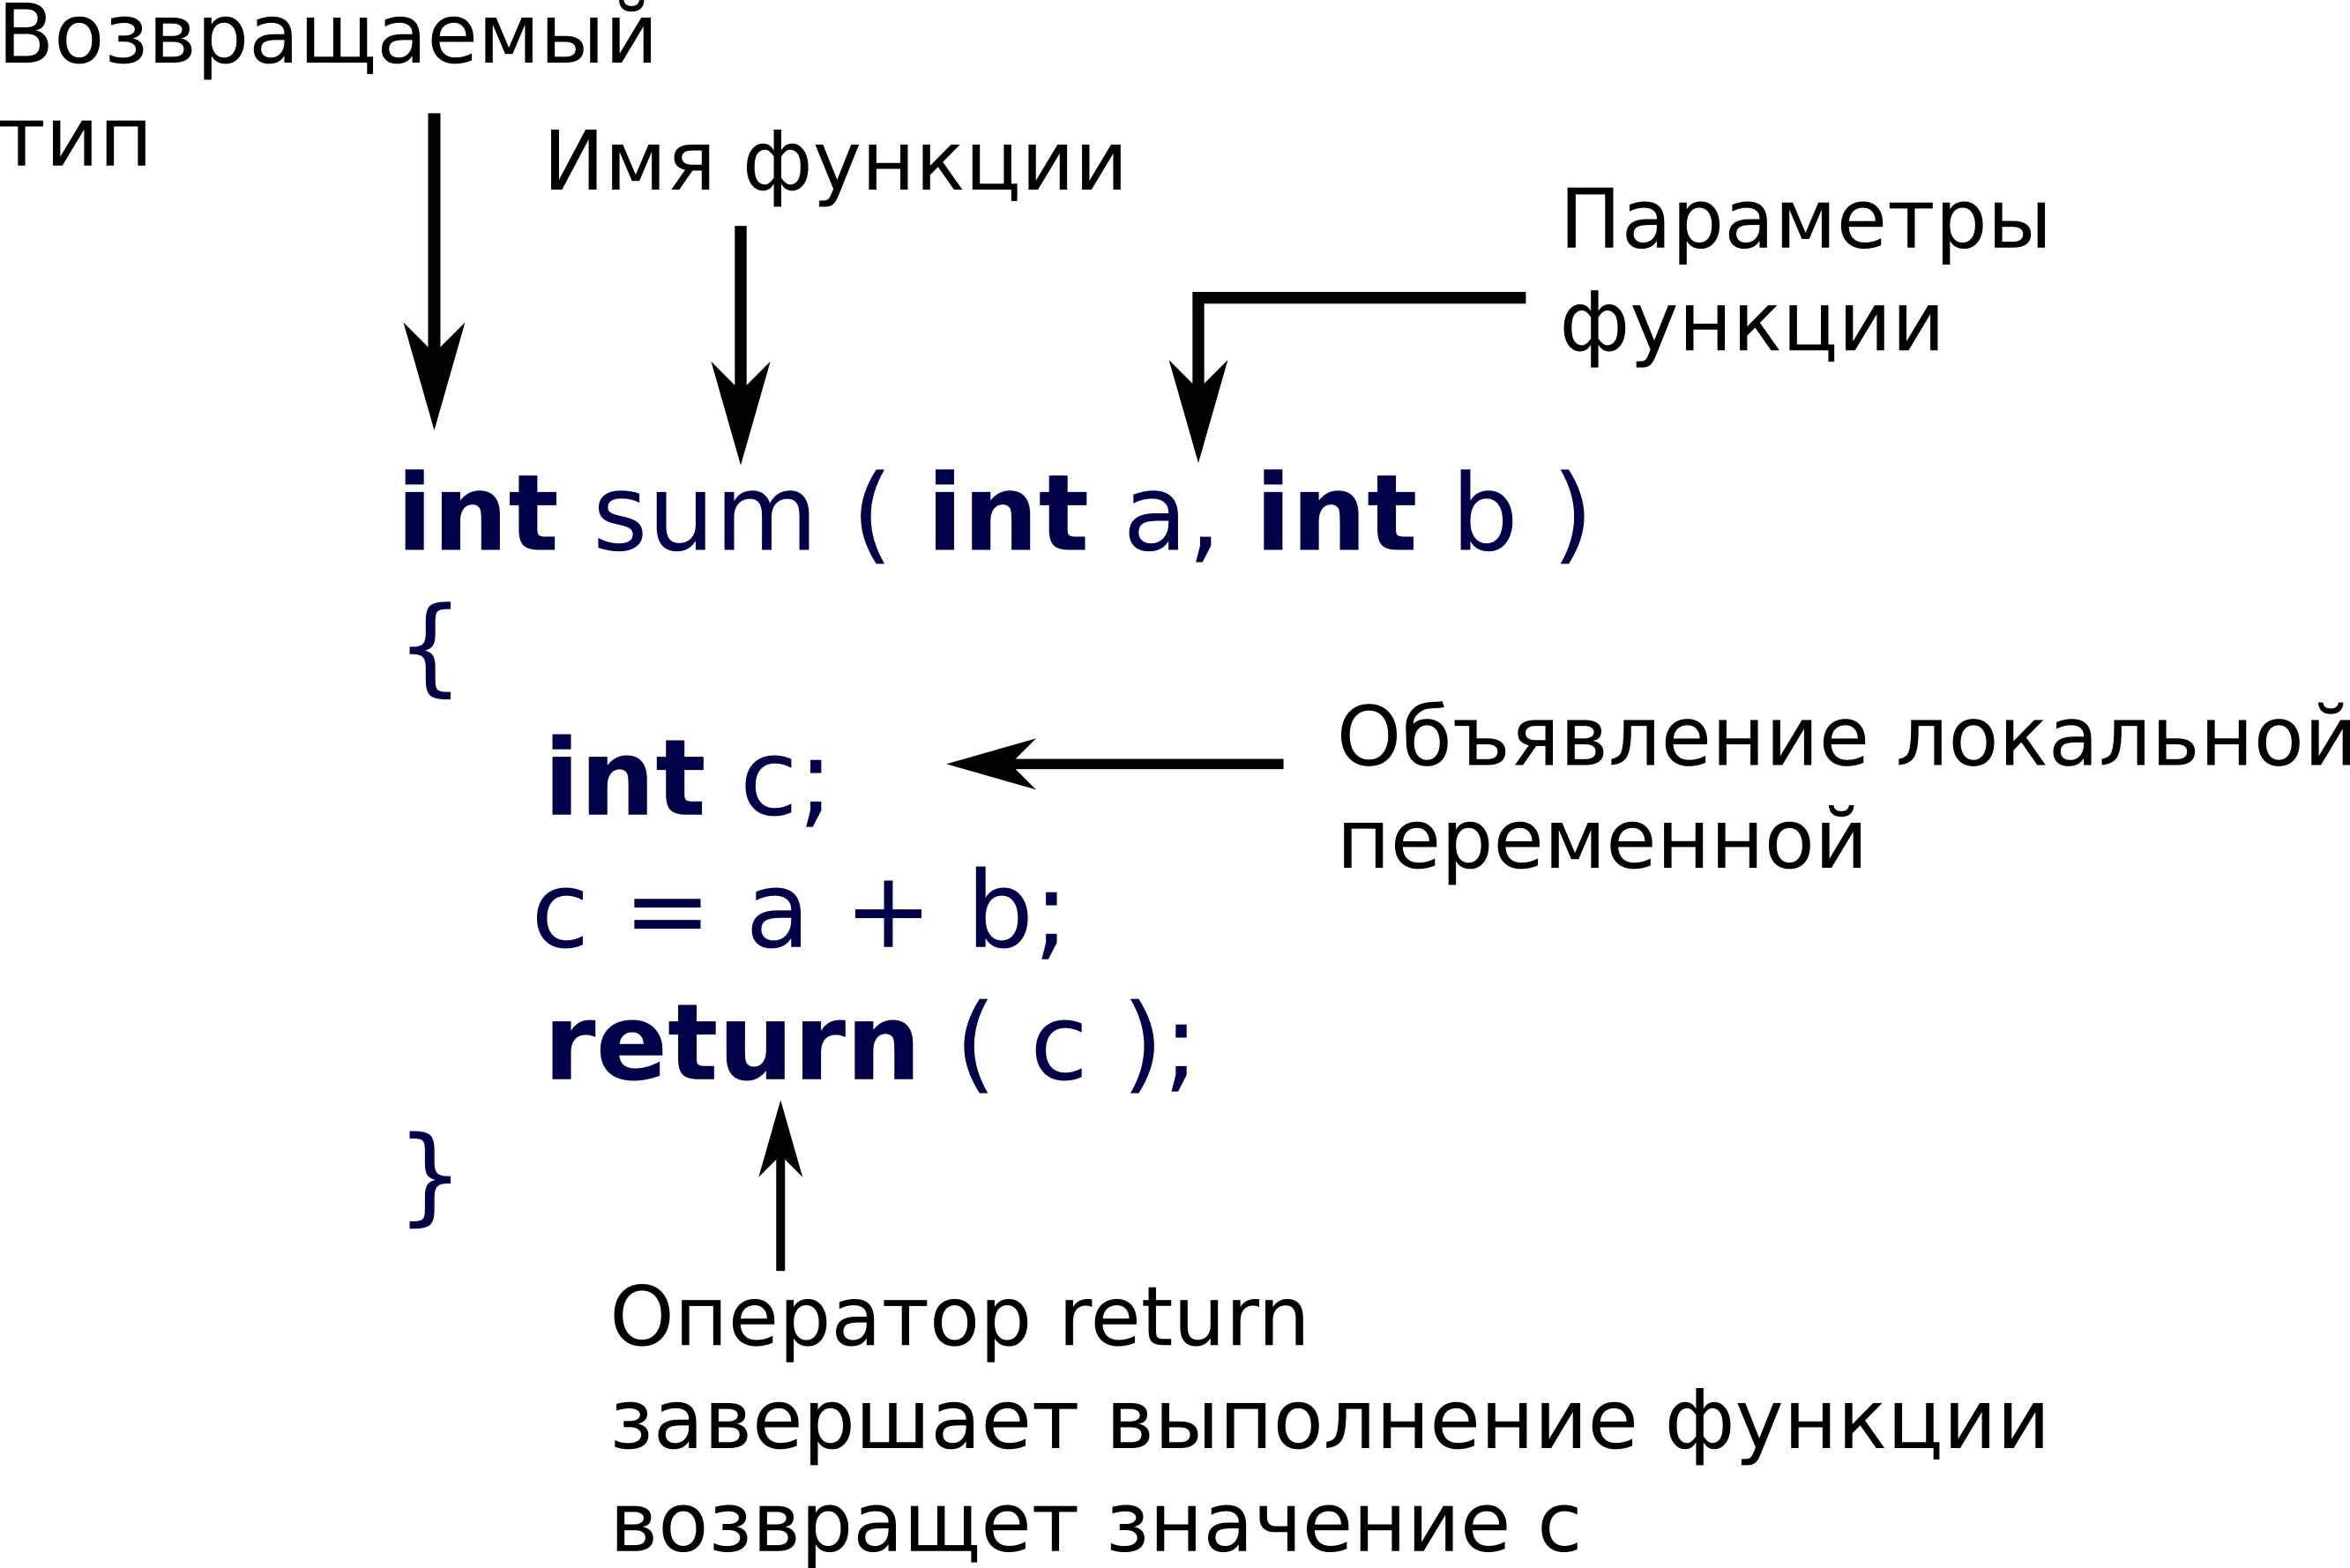
\includegraphics[width=0.8\linewidth]{images/function_syntax.png}
\end{center}
\end{frame}

\begin{frame}[fragile]
\frametitle{Массивы} 
\framesubtitle{Массивы в памяти}
\begin{center}
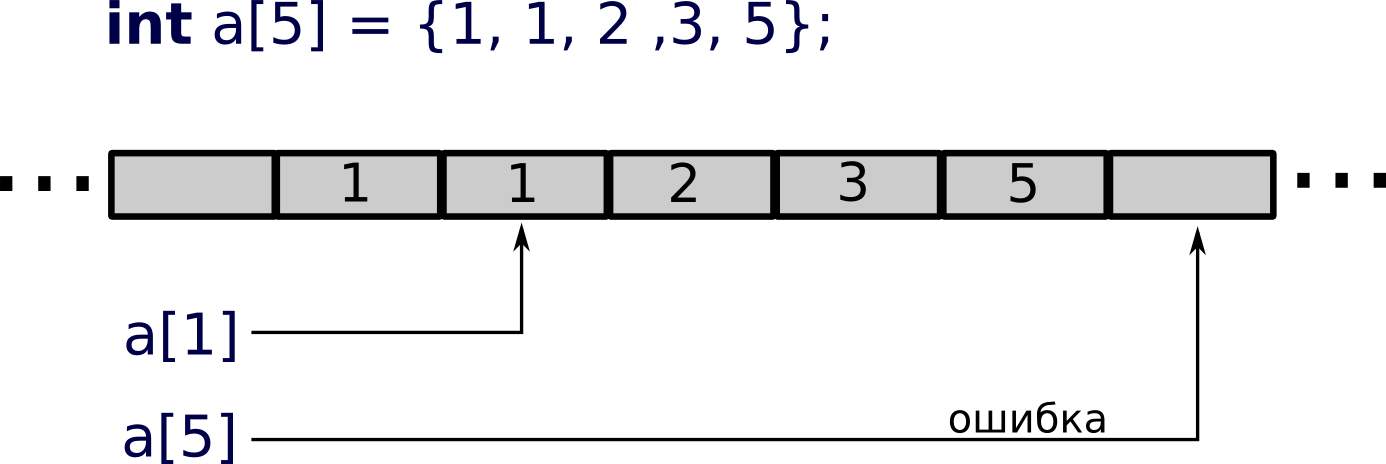
\includegraphics[width=0.95\linewidth]{images/array_in_memory.png}
\end{center}
\end{frame}

\begin{frame}[fragile]
\frametitle{Строки} 
\framesubtitle{Строки в памяти}
\begin{center}
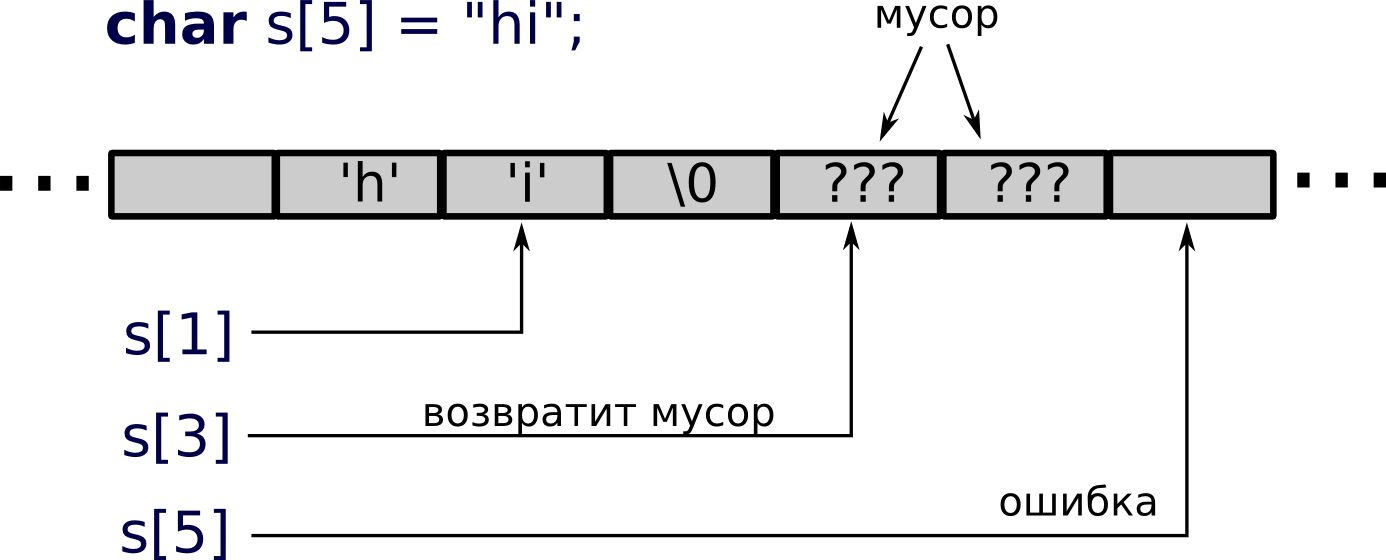
\includegraphics[width=0.95\linewidth]{images/string_in_memory.png}
\end{center}
\end{frame}




\section{Замечания}



\begin{frame}
\frametitle{Базовые типы}
\frametitle{Целочисленные типы} 
Для 64-х битных систем:
\begin{center}
\begin{tabular}{ l c l }
  Название типа & Число бит & Макс. значения \\
  char & 8 & -128..127 или 0..255 \\
  short & 16 & -32768..32767 \\
  int & 32 & $-2 \cdot 10^9$ ..$+2 \cdot 10^9$ \\
  long & 64& $-2^{63}$ ..$+2^{63}-1$ \\
  long long & 64 & $-2^{63}$ ..$+2^{63}-1$ \\
\end{tabular}
\end{center}
\end{frame}

\begin{frame}
\frametitle{Базовые типы}
\frametitle{Беззнаковые целочисленные типы} 
Для 64-х битных систем:
\begin{center}
\begin{tabular}{ l c l }
  Название типа & Число бит & Макс. значения \\
  unsigned char & 8 & 0..255 \\
  unsigned short & 16 & 0..65535 \\
  unsigned int & 32 & $0$ ..$+4 \cdot 10^9$ \\
  unsigned long & 64 & $0$ ..$+2^{64}-1$ \\
  unsigned long long & 64 & $0$ ..$+2^{64}-1$ \\
\end{tabular}
\end{center}
\end{frame}



\begin{frame}
\frametitle{Функции printf() и scanf().}
\begin{center}
\begin{tabular}{ l l l }
  Обозначение & Тип \\
  \%d или \%i & int \\
  \%u & unsigned int \\
  \%l & long \\
  \%ul & unsigned long \\
  \%ll & long long \\
  \%ull & unsigned long long \\
  \%f & float \\
  \%f & double \\
  \%c & char \\
  \%s & Строка\\
\end{tabular}
\end{center}
\end{frame}

\begin{frame}[fragile]
\frametitle{Замечания: for}
\begin{itemize}
\item Опция -std=c99:
\begin{lstlisting}
for (int i = 0; i < N; i++)
\end{lstlisting}
gcc -std=c99 <имя\_файла.c>
\item Цикл for:
\begin{lstlisting}
for (int i = 0; i * i < 1000; i += 5)
\end{lstlisting}
\begin{lstlisting}
for (int i = 10; i > 0; i--)
\end{lstlisting}
\end{itemize}
\end{frame}

\begin{frame}[fragile]
\frametitle{Замечания: математика}
\begin{itemize}
\item Целочисленное деление: (напечатает 2.0)
\begin{lstlisting}
int a = 20, b = 7;
printf("%f\n", a / b); 
\end{lstlisting}
\item Использование библиотеки <math.h>\\
Чтобы использовать математические функции sqrt(), log(), sin(), cos(), tan() и другие нужно подключить
библиотеку: 
\begin{verbatim}
#include <math.h>
\end{verbatim}
и добавить опцию компилятора -lm: \\
gcc -std=c99 -lm <имя\_файла.c>
\end{itemize}
\end{frame}

\begin{frame}[fragile]
\frametitle{Замечания: константы}
\begin{itemize}
\item Директива \#define:
\begin{verbatim}
#define NUMBER_OF_ELEMENTS 100
\end{verbatim}
Заменяет в тексте программы  NUMBER\_OF\_ELEMENTS на 100
\item const:
\begin{verbatim}
const int number_of_elements = 100;
number_of_elements = 200; // Не будет работать
\end{verbatim}
\end{itemize}
\end{frame}

\begin{frame}[fragile]
\frametitle{Замечания: двумерные массивы}
\framesubtitle{Сумма двумерных массивов}
\begin{lstlisting}
int A[100][50], B[100][50], C[100][50];
// ... 
for (int i = 0; i < 100; i++)
     for (int j = 0; j < 50; j++)
     {
         C[i][j] = A[i][j] + B[i][j];
     }
\end{lstlisting}
\end{frame}

\begin{frame}[fragile]
\frametitle{Передача аргументов в функцию}
\framesubtitle{Передача по значению}
\begin{lstlisting}
int min(int a, int b)
{
    if (a < b)
        b = a;
   	return b;
}
int main()
{
    int a = 10, b = 40;
    min(a, b);
    printf("%d\n", b);
}
\end{lstlisting}
\end{frame}

\begin{frame}[fragile]
\frametitle{Передача аргументов в функцию}
\framesubtitle{Передача по значению}
\begin{lstlisting}
int min(int a, int b)
{
    if (a < b)
        b = a;
   	return b;
}
int main()
{
    int x = 10, y = 40;
    min(x, y);
    printf("%d\n", y);
}
\end{lstlisting}
\end{frame}

\begin{frame}[fragile]
\frametitle{Передача аргументов в функцию}
\framesubtitle{Передача по значению}
\begin{lstlisting}
int min(int a, int b)
{
    if (a < b)
        b = a;
   	return b;
}
int main()
{

    min(10, 40);

}
\end{lstlisting}
\end{frame}

\begin{frame}[fragile]
\frametitle{Передача аргументов в функцию}
\framesubtitle{Передача с помощью указателей}
\begin{lstlisting}
void normalize(float* a, float* b)
{
    float sum = *a + *b;
    *a = *a / sum;
    *b = *b / sum;
}
int main()
{
    float x = 10.0, y = 40.0;
    normalize(&x, &y);
    printf("%f\n", y);
}
\end{lstlisting}
\end{frame}


\begin{frame}[fragile]
\frametitle{Указатели и аргументы функций} 
\framesubtitle{Передача по значению}
\begin{center}
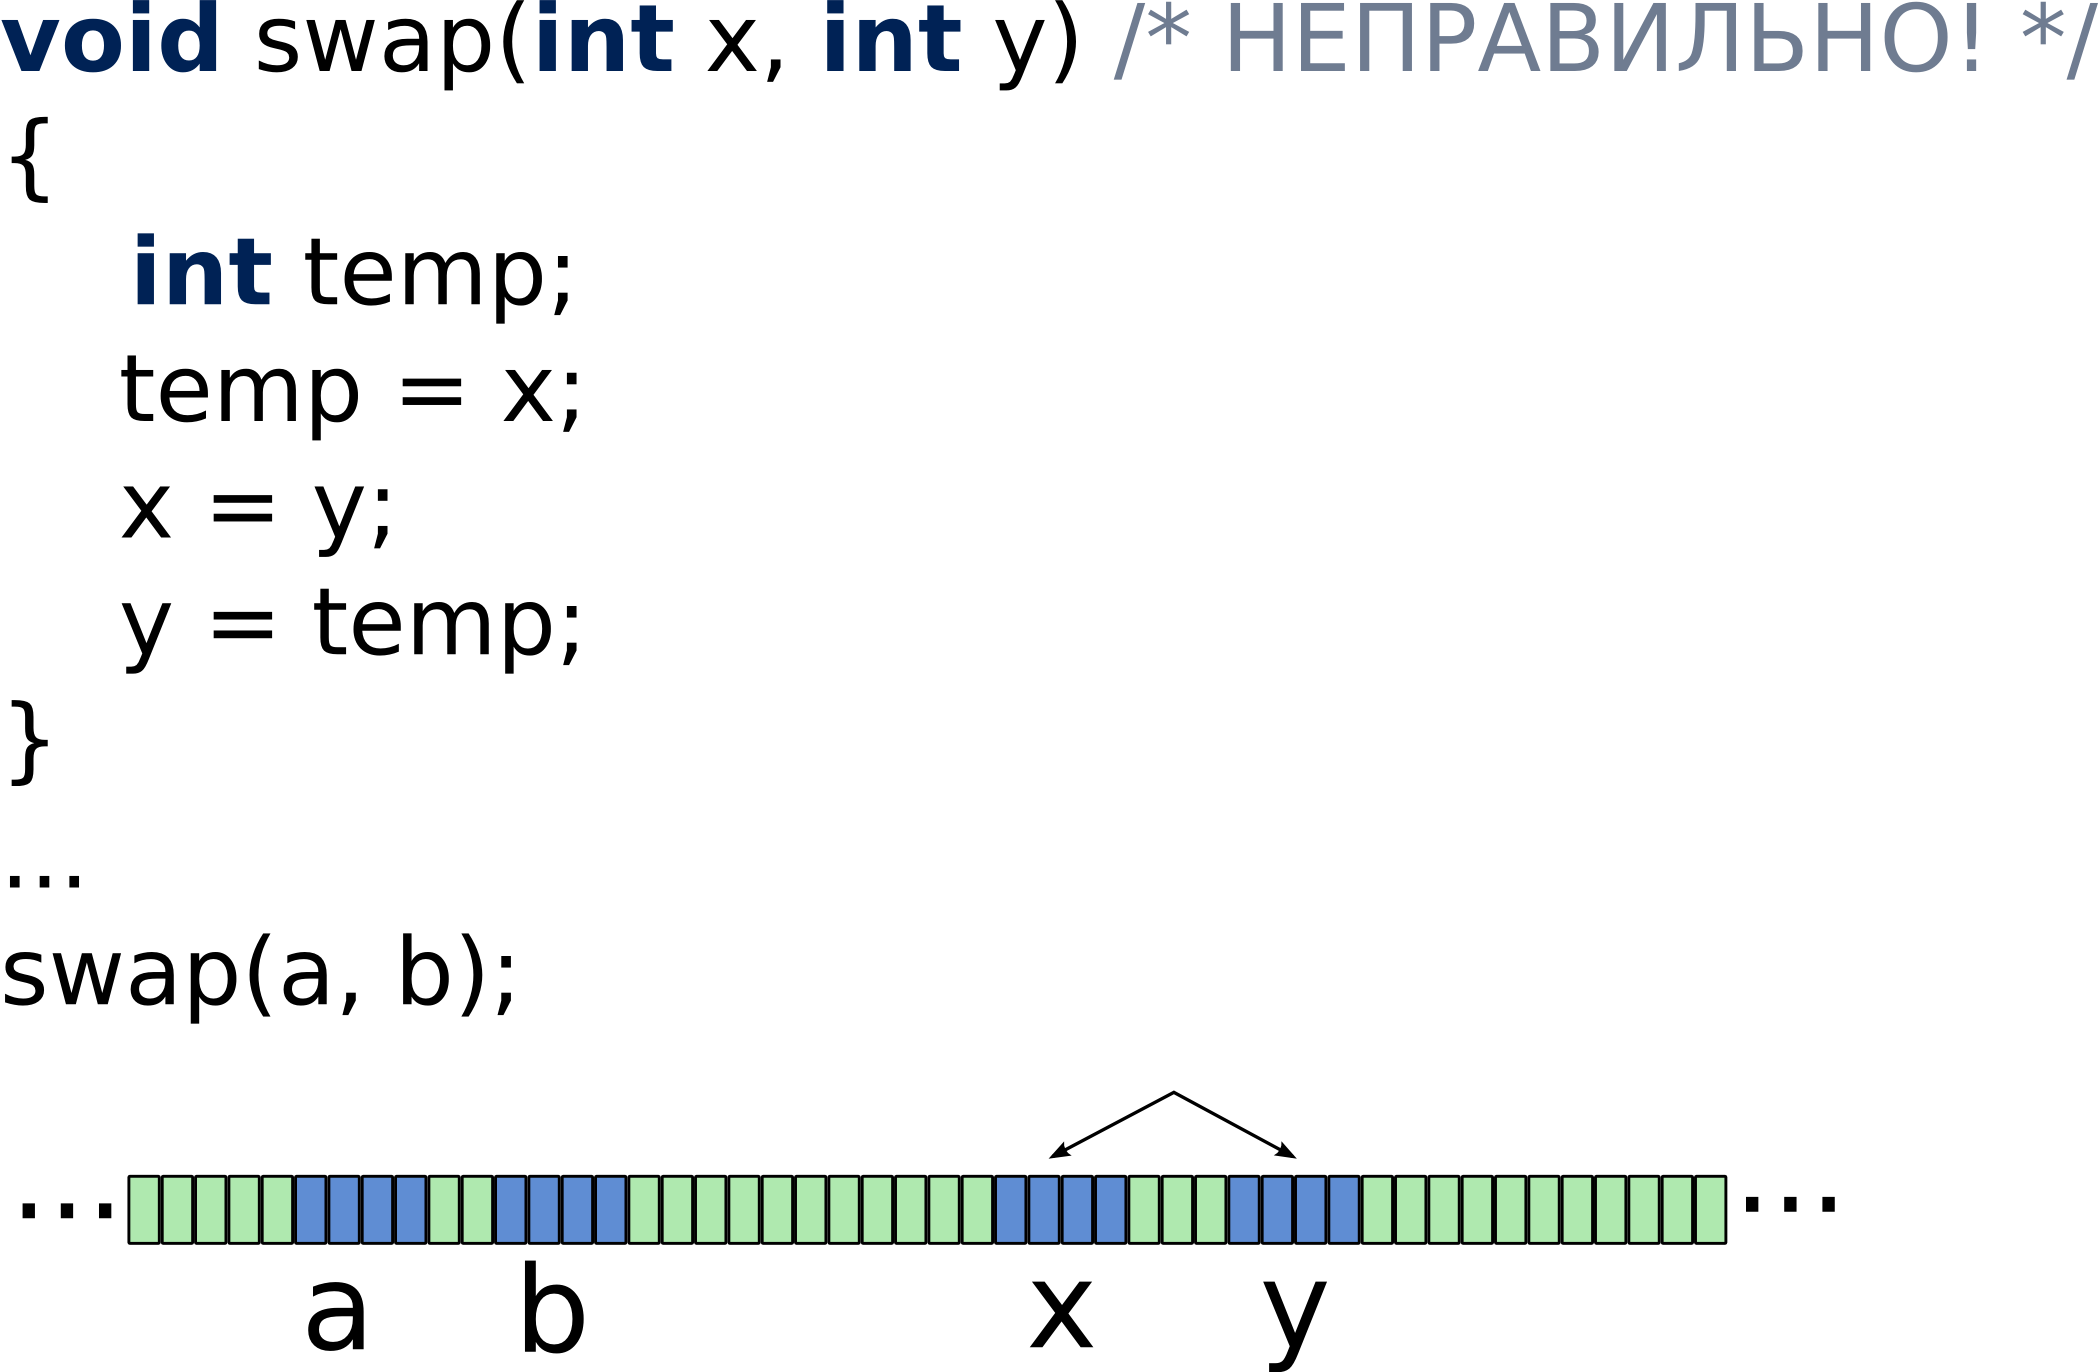
\includegraphics[height=0.55\linewidth]{images/swap_wrong.png}
\end{center}
\end{frame}

\begin{frame}[fragile]
\frametitle{Указатели и аргументы функций} 
\framesubtitle{Передача по адресу}
\begin{center}
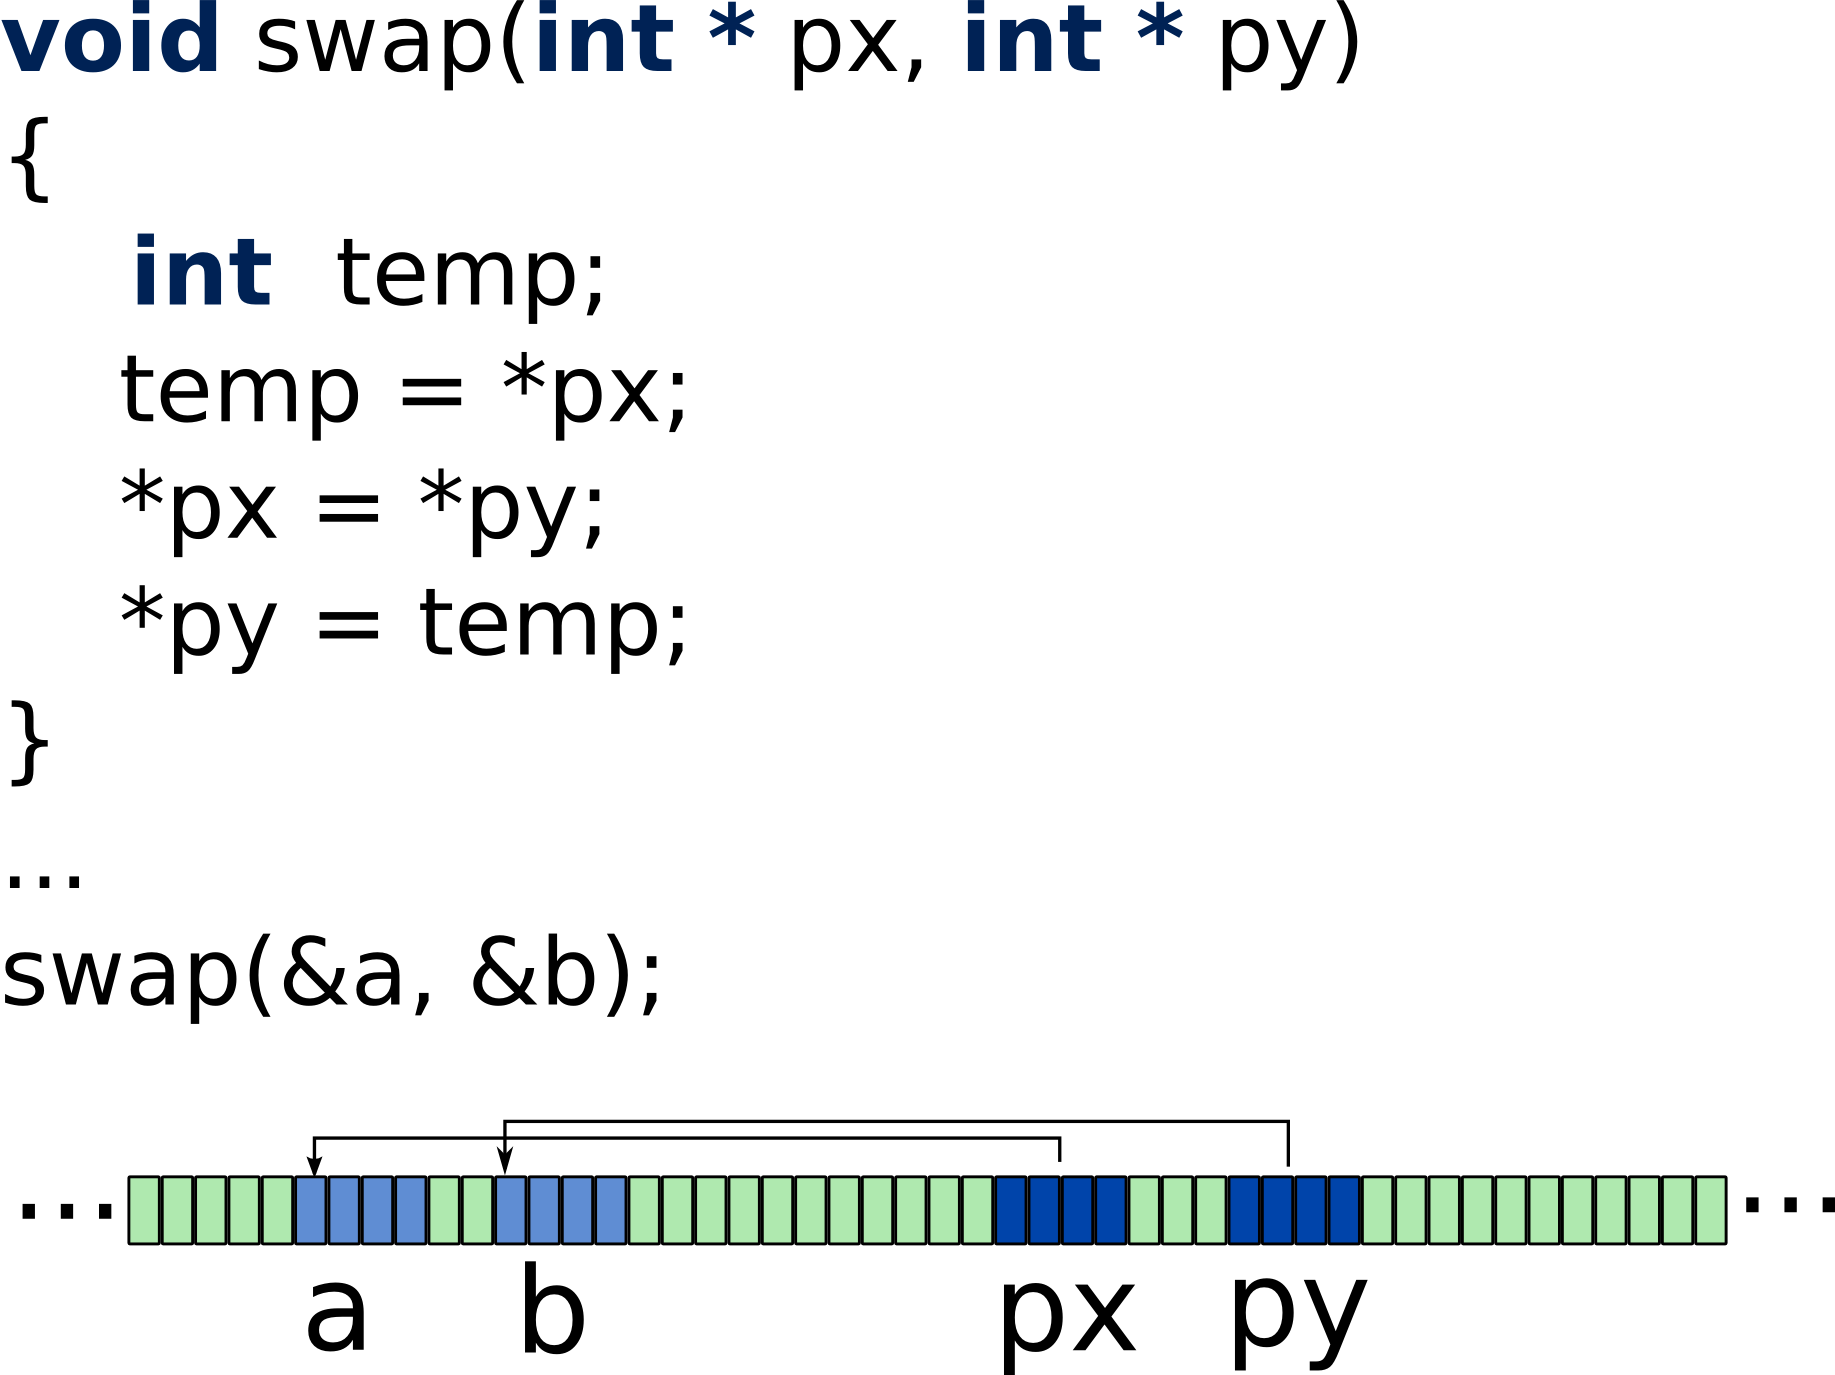
\includegraphics[height=0.55\linewidth]{images/swap_right.png}
\end{center}
\end{frame}








\begin{frame}[fragile]
\frametitle{Передача массивов в функцию}
\framesubtitle{Автоматически передаются с помощью указателей}
\begin{lstlisting}
void add_num(int n, int arr[], int x)
{
    for (int i = 0; i < n; ++i)
        arr[i] += x;
}
int main()
{
    int arr[5] = {1, 5, 7, 3, 16};
    add_num(10, arr, 2);
}
\end{lstlisting}
\end{frame}

\begin{frame}[fragile]
\frametitle{Передача массивов в функцию}
\framesubtitle{Автоматически передаются с помощью указателей}
\begin{lstlisting}
void add_num(int n, int* arr, int x)
{
    for (int i = 0; i < n; ++i)
        arr[i] += x;
}
int main()
{
    int arr[5] = {1, 5, 7, 3, 16};
    add_num(10, arr, 2);
}
\end{lstlisting}
\end{frame}


\begin{frame}[fragile]
\frametitle{Управляющие конструкции} 
\framesubtitle{Оператор break}
\begin{lstlisting}
for (int i = 0; i < 10; ++i)
{
    if (i == 6)
        break
    printf("%d ", i);
}
\end{lstlisting}
Напечатает: 0 1 2 3 4 5
\end{frame}

\begin{frame}[fragile]
\frametitle{Управляющие конструкции} 
\framesubtitle{Оператор continue}
\begin{lstlisting}
for (int i = 0; i < 10; ++i)
{
    if (i == 6)
        continue
    printf("%d ", i);
}
\end{lstlisting}
Напечатает: 0 1 2 3 4 5 7 8 9
\end{frame}


\section{Могли пройти, но не прошли}



\begin{frame}
\frametitle{Управляющие конструкции} 
\framesubtitle{Цикл do while}
\lstinputlisting{./programms/code_do_while.c}
Напечатает 1 2 3 
\end{frame}

\begin{frame}[fragile]
\frametitle{Управляющие конструкции} 
\framesubtitle{Switch}
\begin{lstlisting}
switch(x) {
    case 1:
        printf("It's one!\n");
        break;
    case 2:
        printf("It's two!\n");
        break;
    case 3:
        printf("It's three!\n");
        break;
    default:
        printf("It's something else!\n")
}
\end{lstlisting}
\end{frame}

\begin{frame}[fragile]
\frametitle{Перечисляемый тип enum} 
\begin{lstlisting}
enum day{Mon, Tue, Wed, Thur, Fri, Sat, Sun};
// Mon = 0, Tue = 1, Wed = 2, ...
int main()
{
    enum day x;
    x = Wed;
    printf("%d", x);
} 
\end{lstlisting}
Напечатает 2
\end{frame}

\begin{frame}[fragile]
\frametitle{Ещё} 
\begin{itemize}
\item Тернарный оператор: <условие> ? <\#1> : <\#2>\\
\begin{lstlisting}
int b = a > 0 ? a : -a;
\end{lstlisting}
\item Запретный оператор goto \\
\begin{center}

\includegraphics[width=0.99\linewidth]{images/goto.png}
\end{center}
\end{itemize}
\end{frame}



\begin{frame}[fragile]
\frametitle{Тренировка перед контрольной работой} 
http://style.vdi.mipt.ru/  -- тренировка перед контрольной работой
\end{frame}



\end{document}
